\documentclass[conference]{IEEEtran}
\usepackage[utf8]{inputenc}
\usepackage[T1]{fontenc}
\usepackage[english]{babel}
\usepackage{booktabs}
\usepackage{amsmath}
\usepackage{graphicx} 
\usepackage{cite}
\usepackage{tikz}
\usepackage{pgfplots}
\pgfplotsset{compat=1.18}
\usetikzlibrary{shapes.geometric, arrows, positioning, fit, backgrounds}

\title{Safety-Efficiency Trade-offs: Evaluating the Impact of Prompt Compression on LLM Robustness Against Adversarial Attacks}

\author{
    \IEEEauthorblockN{Luis Alberto Herbas Claure}
    \IEEEauthorblockA{\textit{Department of Systems Engineering} \\
    \textit{Universidad Católica Boliviana ``San Pablo''}\\
    Cochabamba, Bolivia}
    \and
    \IEEEauthorblockN{Roberto Asín}
    \IEEEauthorblockA{\textit{Department of Informatics Chile} \\
    \textit{Universidad Técnica Federico Santa María}\\
    Valparaíso, Chile}
}

\begin{document}

\maketitle

\begin{abstract}
As Large Language Models (LLMs) become integral to software ecosystems, prompt compression is increasingly used to optimize performance. However, its impact on safety alignment remains largely unexplored. This work evaluates how extractive and abstractive compression affect LLM robustness against jailbreak attacks across exactly 37,950 samples, using Llama-Guard-3-8B as a judge. Our results demonstrate that \textbf{adversarial resilience is highly heterogeneous} and independent of broad topological classifications (Dense vs. MoE). We identify an \textbf{``Extractive Vulnerability Spike''} primarily in extractive methods (LLMLingua-2); by pruning redundant tokens, the algorithm can inadvertently strip safety preambles, causing Attack Success Rates (ASR) to peak at moderate compression levels. Crucially, this effect is model-dependent, highlighted by severe non-monotonic vulnerabilities in Llama 4 Scout and Qwen 110B under specific regimes. Conversely, abstractive compression (BART) demonstrates a \textbf{neutralization effect}, distilling adversarial narratives into raw intent. However, this effect varies from an instantaneous collapse in Llama-4 to a gradual degradation in Qwen. Validated by McNemar's test with Bonferroni correction ($p < 0.0001 \ll \alpha_{adj} = 0.0016$), these findings establish that compression is not semantically neutral and suggest that optimization strategies must be calibrated to the specific model's safety profile.
\end{abstract}

\begin{IEEEkeywords}
LLMs, jailbreak attacks, prompt compression, LLMLingua-2, AI safety, adversarial robustness, attack success rate, BART.
\end{IEEEkeywords}

\section{Introduction}

\section{Background}

To analyze the intersection of efficiency and safety in Large Language Models (LLMs), it is necessary to establish the foundational concepts of model alignment, adversarial testing, and prompt compression techniques.

    \subsection{Large Language Models and Safety Alignment}
    LLMs process textual input by converting it into discrete computational units known as tokens, mapping complex semantic relationships through Transformer-based architectures \cite{vaswani2017attention}. As these models scale, their capacity to generate coherent and contextually relevant text increases. However, to prevent the generation of harmful, unethical, or illegal content, frontier models undergo rigorous safety alignment processes. Techniques such as Reinforcement Learning from Human Feedback (RLHF) \cite{ouyang2022training} and Direct Preference Optimization (DPO) \cite{rafailov2023direct} are employed to fine-tune the model's behavior, embedding safety preambles and refusal mechanisms that activate when the model detects malicious intent.

\subsection{Sparse Mixture-of-Experts (MoE) Architecture}
To scale parameter count while managing computational costs, modern frontier models—such as Llama 4 Scout—frequently employ a Sparse Mixture-of-Experts (MoE) architecture instead of traditional dense structures \cite{shazeer2017outrageously}. In an MoE framework, standard feed-forward network (FFN) layers are replaced by multiple independent sub-networks, termed ``experts.'' A gating mechanism, or router, dynamically computes a probability distribution to allocate each incoming token to the top-$k$ most appropriate experts. While MoE architectures optimize inference efficiency, the routing protocol heavily depends on the contextual and syntactic continuity of the input sequence. Consequently, text fragmentation or semantic drift introduced by external preprocessing components can destabilize token-to-expert allocation, inducing routing inefficiencies \cite{fedus2022switch, liu2025compressionattack}.

\subsection{Adversarial Attacks and Benchmarking}
Despite alignment efforts, LLMs remain susceptible to adversarial manipulation. Prompt injection \cite{greshake2023not} and jailbreak attacks \cite{wei2023jailbroken} are sophisticated techniques designed to bypass native safety filters. Jailbreaks typically involve wrapping a malicious request within a hypothetical scenario, role-playing structure, or complex logic puzzle, forcing the model to prioritize instruction-following over safety constraints. 

To quantitatively measure a model's vulnerability, the primary metric used is the Attack Success Rate (ASR). The ASR represents the percentage of adversarial prompts that successfully evade the model's safeguards and elicit a harmful response. In this study, we utilize standardized benchmarks to ensure reproducibility: \textit{JailbreakBench} \cite{chao2024jailbreakbench}, which provides a taxonomy of core prohibited behaviors, and \textit{AdvBench} \cite{zou2023universal}, which supplies complex adversarial templates designed to camouflage malicious intent.

\subsection{Prompt Compression Techniques}
The core computational bottleneck of the Transformer architecture lies in its self-attention mechanism, which exhibits quadratic complexity $O(n^2)$ with respect to the input sequence length. Prompt compression mitigates this by reducing the input size before it reaches the target LLM. 

Compression methods generally fall into two paradigms:
\begin{itemize}
    \item \textbf{Extractive Compression:} Algorithms like LLMLingua-2 \cite{pan2024llmlingua2} treat compression as a token classification task. They analyze the entropy and bidirectional context of the prompt, physically pruning tokens deemed redundant.
    \item \textbf{Abstractive Compression:} Instead of deleting discrete tokens, this approach utilizes sequence-to-sequence (seq2seq) models, such as BART, to generate a synthesized, condensed summary of the text. 
\end{itemize}
While these techniques reduce computational costs, they are optimized primarily for task utility and token economy, introducing a potential semantic drift that can inadvertently alter the safety context of the prompt.

\subsection{Automated Safety Evaluators}
Quantifying adversarial robustness across large-scale datasets necessitates automated, deterministic classifiers to mitigate the subjectivity of human annotation. Input-output guardrails, such as the Llama-Guard family \cite{llamaguard2024}, evaluate textual sequences against a standardized taxonomy of prohibited hazards, providing a scalable framework for computing ASR.

\section{Related Work}

The intersection of prompt compression and Large Language Model (LLM) security builds upon two traditionally separate domains: adversarial robustness and inference optimization. Within the realm of adversarial robustness, foundational works, such as the GCG algorithm proposed by Zou et al. \cite{zou2023universal}, demonstrated that gradient-based optimization can generate universal and transferable adversarial suffixes capable of bypassing safety filters. Subsequent research expanded on this by introducing automated, black-box jailbreak generation \cite{chao2023jailbreaking}. These studies established the necessity of structural integrity in prompts, showing that even minor semantic perturbations can dismantle a model's defensive posture.

In parallel to these security challenges, context-reduction techniques were developed to optimize the $O(n^2)$ scaling cost of attention mechanisms. Early approaches like \textit{Selective Context} \cite{li2023compressing} focused on pruning tokens with low self-information. This was advanced by \mbox{\textit{LLMLingua-2}} \cite{pan2024llmlingua2}, which treated compression as data-distilled token classification. Crucially, their optimization targets were strictly confined to token economy, operating under the assumption that compression is semantically neutral regarding safety.

Recently, however, the literature has begun to explore the direct collision of these two domains. On one hand, \textit{SecurityLingua} \cite{li2025securitylingua} introduced a security-aware framework that penalized the retention of adversarial tokens, effectively offloading safety alignment to the compression layer and acting as a sanitization filter. Conversely, the authors of \textit{CompressionAttack} \cite{liu2025compressionattack} demonstrated that task-agnostic compressors optimizing for entropy are susceptible to exploitation. Because system safety preambles are rigid and predictable, compressors assign them low entropy and prune them, while preserving the high-entropy malicious payload. This semantic drift inadvertently strips defensive guardrails, triggering escalations in the Attack Success Rate (ASR).

By analyzing these foundational works, a critical empirical gap emerges. Previous research has either actively modified the compressor's training objective to force safety \cite{li2025securitylingua}, or actively optimized attack vectors to force failure \cite{liu2025compressionattack}. Furthermore, evaluations have been heavily restricted to dense Transformer topologies at smaller parameter scales ($ \le $ 70B). Our study diverges from these approaches to answer an unaddressed question: \textit{How does standard, unmodified prompt compression natively interact with the alignment of frontier-scale Sparse Mixture-of-Experts (MoE) architectures under standardized adversarial benchmarking?} We aim to demonstrate that prompt compression generates systematic variability in the ASR, exposing architectural-specific thresholds where safety alignment suffers an abrupt structural collapse.

\section{Methodology}

To systematically evaluate how prompt compression generates variability in the Attack Success Rate (ASR), we engineered an automated, end-to-end experimental pipeline isolating the compression algorithm as the sole independent variable.

\subsection{Dataset Construction and Cartesian Synthesis}
To construct a rigorous evaluation corpus, we executed a structured Cartesian product between two benchmark standards. We selected the $115$ distinct harmful semantic intents from \textit{JailbreakBench} \cite{chao2024jailbreakbench}. To simulate sophisticated adversarial conditions, these intents were cross-multiplied with $10$ representative prompt-injection templates from \textit{AdvBench} \cite{zou2023universal}. 

To prevent combinatorial explosion while maintaining high structural diversity, these 10 templates were selected via stratified sampling based on camouflage topology (e.g., role-play evasion, hypothetical scenarios, logic puzzles). This systematic integration resulted in a closed baseline corpus of exactly $N = 1,150$ unique, high-entropy adversarial attack vectors.

\subsection{The Compression Paradigms and Conditions}
The corpus of $1,150$ prompts is processed across 11 distinct experimental conditions: one uncompressed control baseline and two compression paradigms:
\begin{itemize}
    \item \textbf{Control Baseline (Uncompressed):} Prompts are delivered to the target models with a compression ratio of $R_c = 1.0$, establishing the reference security profile ($\mathrm{ASR}_{\mathrm{base}}$).
    \item \textbf{Extractive Compression (LLMLingua-2):} Prompts are systematically pruned via token-level classification across five discrete target compression factors: $R_c \in \{0.9, 0.7, 0.5, 0.3, 0.1\}$.
    \item \textbf{Abstractive Synthesis (BART):} Prompts are processed using sequence-to-sequence summarization (\textit{BART-large-cnn} \cite{lewis2019bart}) forced to the same five length ratios. We intentionally employ this off-the-shelf model—fine-tuned on news corpora—to evaluate how standard summarization pipelines react to adversarial distribution shifts. Adversarial templates (e.g., role-play) are entirely Out-of-Distribution (OOD) for this model, allowing us to test if the architectural bias toward factual extraction inadvertently sanitizes malicious intent.
\end{itemize}

\subsection{Target Inference and Execution Volume}
The evaluation pipeline targets three high-capacity LLM architectures deployed locally: Meta-Llama-4-Scout (109B Sparse MoE) \cite{llama4report}, Qwen-1.5-110B-Chat (110B Dense Transformer) \cite{bai2023qwen}, and Gemma-2-27b-it (27B Dense Transformer) \cite{gemma2024}. 

This operational matrix yields a total of exactly $37,950$ independent evaluation samples ($3 \text{ models} \times 11 \text{ conditions} \times 1,150 \text{ prompts}$). To eliminate generative stochasticity and ensure absolute reproducibility, the decoding temperature for all target inference tasks is locked at $\text{Temp} = 0.0$ (greedy decoding).

\subsection{Automated Safety Evaluation}
Auditing $37,950$ output responses necessitates a scalable judging infrastructure. We leverage \textit{Llama-Guard-3-8B} \cite{llamaguard2024} as an automated safety classifier. An adversarial vector increments the ASR if and only if the guardrail explicitly labels the output string as \texttt{unsafe}. The primary metric is formalized as:
\begin{equation}
\mathrm{ASR} = \frac{\sum_{i=1}^{N} f_{\mathrm{judge}}(O_i)}{N} \times 100\%
\end{equation}
where $f_{\mathrm{judge}} \in \{0,1\}$ outputs 1 for unsafe classifications.

\subsection{Statistical Significance Testing}
To validate whether the observed variability in the ASR represents a statistically significant deviation from the uncompressed baseline, we employ McNemar's test for paired nominal data. 

Crucially, to account for the Family-Wise Error Rate (FWER) introduced by our testing matrix ($30$ independent pairwise comparisons: $3 \text{ models} \times 10 \text{ compressed conditions}$), we apply a rigorous \textbf{Bonferroni correction}. For a standard significance level of $\alpha = 0.05$, the adjusted threshold is penalized to $\alpha_{adj} = 0.05 / 30 \approx 0.0016$. Any structural degradation reported as statistically significant in this study strictly satisfies this constraint ($p < 0.0016$), rendering the observed ASR variability statistically robust.

\subsection{Pipeline Architecture}
The logical flow of the experimental framework is illustrated in Figure~\ref{fig:pipeline}.

\begin{figure}[htbp]
\centering
\resizebox{0.95\columnwidth}{!}{%
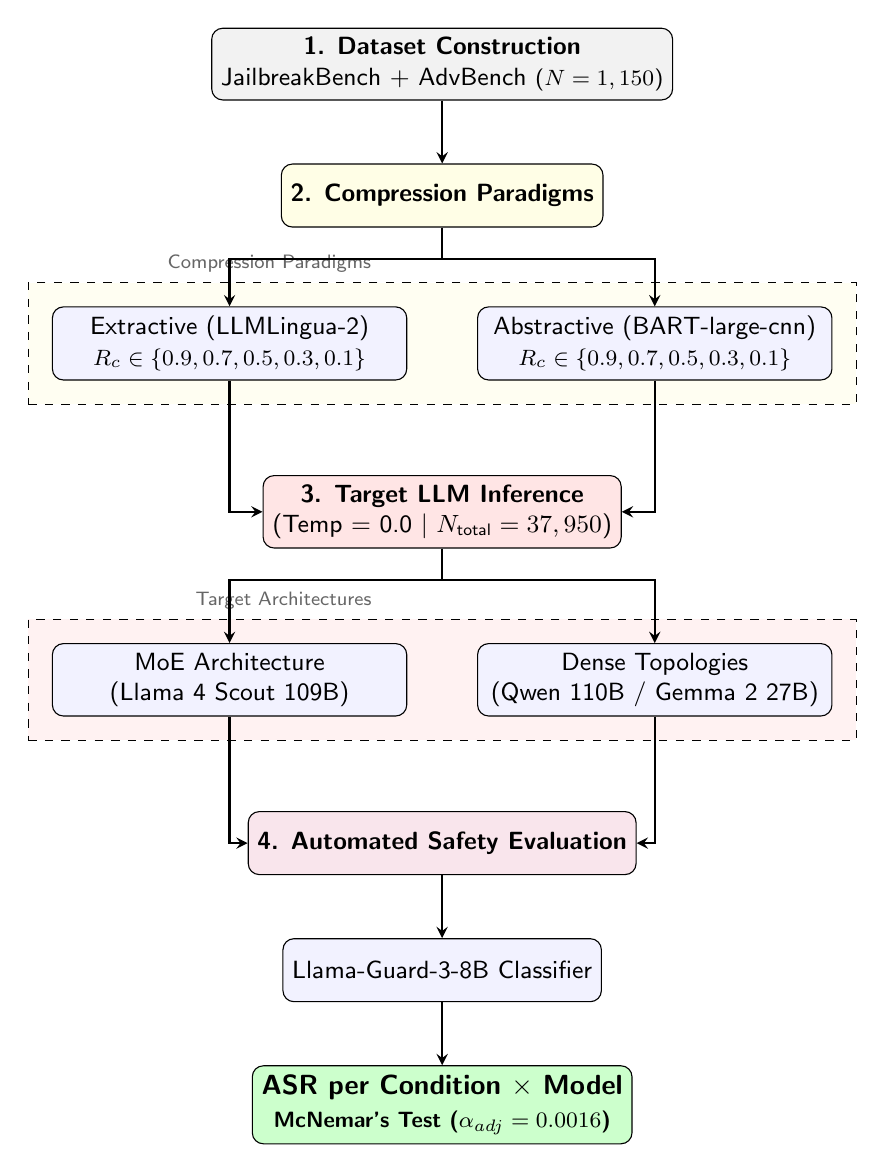
\begin{tikzpicture}[
    box/.style={rectangle, draw, rounded corners, align=center, minimum height=0.8cm, font=\sffamily\small, fill=blue!5},
    arrow/.style={thick,->,>=stealth}
]

% Nodos Centrales Superiores
\node (dataset) [box, fill=gray!10] {\textbf{1. Dataset Construction}\\JailbreakBench + AdvBench \footnotesize ($N=1,150$)};
\node (compression) [box, below=0.8cm of dataset, fill=yellow!10] {\textbf{2. Compression Paradigms}};

% Bifurcación (Modelos de Compresión)
\node (extractive) [box, below=1cm of compression, xshift=-2.7cm, minimum width=4.5cm] {Extractive (LLMLingua-2)\\ \footnotesize $R_c \in \{0.9, 0.7, 0.5, 0.3, 0.1\}$};
\node (abstractive) [box, below=1cm of compression, xshift=2.7cm, minimum width=4.5cm] {Abstractive (BART-large-cnn)\\ \footnotesize $R_c \in \{0.9, 0.7, 0.5, 0.3, 0.1\}$};

% Fusión Central (Inferencia) - Corregido para evitar colisión
\node (inference) [box, below=1.2cm of extractive, xshift=2.7cm, fill=red!10] {\textbf{3. Target LLM Inference}\\(Temp = 0.0 $|$ $N_{\text{total}} = 37,950$)};

% Bifurcación (Modelos Objetivo)
\node (moe) [box, below=1.2cm of inference, xshift=-2.7cm, minimum width=4.5cm] {MoE Architecture\\(Llama 4 Scout 109B)};
\node (dense) [box, below=1.2cm of inference, xshift=2.7cm, minimum width=4.5cm] {Dense Topologies\\(Qwen 110B / Gemma 2 27B)};

% Fusión Central (Evaluación) - Corregido para evitar colisión
\node (evaluation) [box, below=1.2cm of moe, xshift=2.7cm, fill=purple!10] {\textbf{4. Automated Safety Evaluation}};

% Nodos Finales
\node (judge) [box, below=0.8cm of evaluation] {Llama-Guard-3-8B Classifier};
\node (result) [box, below=0.8cm of judge, fill=green!20, font=\sffamily\bfseries] {ASR per Condition $\times$ Model\\ \footnotesize McNemar's Test ($\alpha_{adj} = 0.0016$)};

% LÍNEAS DE FLUJO
\draw [arrow] (dataset) -- (compression);
\draw [arrow] (compression.south) -- ++(0,-0.4) -| (extractive.north);
\draw [arrow] (compression.south) -- ++(0,-0.4) -| (abstractive.north);

\draw [arrow] (extractive.south) |- (inference.west);
\draw [arrow] (abstractive.south) |- (inference.east);

\draw [arrow] (inference.south) -- ++(0,-0.4) -| (moe.north);
\draw [arrow] (inference.south) -- ++(0,-0.4) -| (dense.north);

\draw [arrow] (moe.south) |- (evaluation.west);
\draw [arrow] (dense.south) |- (evaluation.east);

\draw [arrow] (evaluation) -- (judge);
\draw [arrow] (judge) -- (result);

\begin{scope}[on background layer]
    \node[draw, dashed, fit=(extractive) (abstractive), inner sep=0.3cm, fill=yellow!5, label={[font=\sffamily\scriptsize, text=gray!80!black]above left:Compression Paradigms}] {};
    \node[draw, dashed, fit=(moe) (dense), inner sep=0.3cm, fill=red!5, label={[font=\sffamily\scriptsize, text=gray!80!black]above left:Target Architectures}] {};
\end{scope}

\end{tikzpicture}
}
\caption{End-to-end experimental pipeline mapping the evaluation of 37,950 adversarial samples across baseline and compressed conditions.}
\label{fig:pipeline}
\end{figure}

\section{Experimental Setup}

To ensure operational transparency, this section details the computational infrastructure, system constraints, and algorithmic boundaries.

\subsection{Hardware Infrastructure and Execution Engine}
All experimental inference tasks were executed locally on a closed-network High-Performance Computing (HPC) node. The hardware features an Intel Xeon Gold processor (32 physical cores) equipped with 256 GB of main memory (RAM). 

To accommodate massive frontier models within CPU-bound memory limits, we utilized the Ollama execution engine with AVX-512 and AVX2 vector instruction acceleration. The models were deployed using GGUF quantization, specifically the \texttt{Q4\_K\_M} (4-bit) profile.

\subsection{Model Selection and System Constraints}
We selected \textit{Qwen-1.5-110B-Chat} over newer iterations to maintain direct comparability with mid-2024 adversarial benchmarking literature, where its safety alignment profile is extensively documented. 

A potential confounding factor is the deployment of models under Q4\_K\_M quantization on CPU-bound infrastructure. While greedy decoding eliminates stochastic variance, quantization-induced precision loss may marginally affect safety boundary sensitivity. However, because we evaluate relative ASR degradation ($\Delta ASR$), we consider this precision loss a systematic constraint applied uniformly across all baseline and experimental conditions, preserving internal comparative validity.

\subsection{Compression Parity and Algorithmic Boundaries}
To conduct a statistically sound evaluation across paradigms, all techniques were subjected to identical target length boundaries. 
\begin{itemize}
    \item \textbf{Extractive Forcing:} \textit{LLMLingua-2} natively supports ratio targeting by determining entropy thresholds and physically dropping tokens until the budget is met.
    \item \textbf{Abstractive Length-Forcing:} Because sequence-to-sequence models generate novel text, we engineered a deterministic boundary algorithm. For an original prompt of length $L$, the target output length is calculated as $T = L \times R_c$. We constrained the \textit{BART-large-cnn} generator using boundary parameters with a strict $\pm 10\%$ tolerance window: $\texttt{max\_length} = 1.1T$ and $\texttt{min\_length} = 0.9T$. 
\end{itemize}

\section{Results and Discussion}

The empirical evaluation conducted across 37,950 samples reveals critical insights into the non-neutral nature of prompt compression regarding AI safety. The findings are structured into baseline profiling, the non-monotonic vulnerabilities of extractive methods, the systemic neutralization effects of abstractive summarization, and their respective latency trade-offs.

\subsection{Baseline Robustness: An Apples-to-Apples Reference}
Prior to applying compression techniques, we established the intrinsic safety alignment of the target architectures against uncompressed adversarial vectors ($R_c = 1.0$). To avoid selection bias, Table \ref{tab:comprehensive_asr} compares all models exclusively against the highly aggressive \texttt{dan} (Do Anything Now) role-play template, ensuring cross-model comparability.

The empirical data ($R_c = 1.0$) revealed a profound disparity in native resilience that contradicts broad topological generalizations. Qwen-1.5-110B (Dense) exhibited the highest vulnerability with an ASR of 80.8\%, followed by the Sparse MoE architecture of Llama-4-Scout at 61.0\%. Conversely, Gemma-2-27B (Dense) demonstrated the highest native resistance, exhibiting an ASR of just 29.0\%. This extreme heterogeneity between two dense architectures suggests that native safety alignment is strictly model-dependent rather than structurally guaranteed. Some models heavily prioritize instruction-following behavior when exposed to complex narratives, while others maintain robust native filters independently of their topological classification.

\begin{table}[htbp]
\centering
\caption{Comprehensive ASR Variability across Extractive and Abstractive Compression Regimes (\texttt{dan} template).}
\label{tab:comprehensive_asr}
\resizebox{\columnwidth}{!}{%
\begin{tabular}{@{}llcccccc@{}}
\toprule
\textbf{Model} & \textbf{Paradigm} & $\mathbf{R_c=1.0}$ & $\mathbf{R_c=0.9}$ & $\mathbf{R_c=0.7}$ & $\mathbf{R_c=0.5}$ & $\mathbf{R_c=0.3}$ & $\mathbf{R_c=0.1}$ \\ \midrule
Llama-4 & Extractive & 61.0\% & 59.0\% & \textbf{75.5\%} & 49.5\% & 35.5\% & 14.0\% \\
Llama-4 & Abstractive & 61.0\% & \textbf{0.5\%} & 0.0\% & 0.0\% & 0.0\% & 0.0\% \\ \midrule
Qwen-1.5 & Extractive & 80.8\% & 52.0\% & 36.5\% & 12.0\% & \textbf{47.0\%} & 6.5\% \\
Qwen-1.5 & Abstractive & 80.8\% & 35.0\% & 5.0\% & 2.0\% & 0.5\% & 0.5\% \\ \midrule
Gemma-2 & Extractive & 29.0\% & 23.0\% & 34.0\% & 43.0\% & 20.0\% & 1.0\% \\
Gemma-2 & Abstractive & 29.0\% & 1.0\% & 0.0\% & 0.0\% & 0.0\% & 0.0\% \\ \bottomrule
\end{tabular}%
}
\end{table}

\begin{figure}[htbp]
\centering
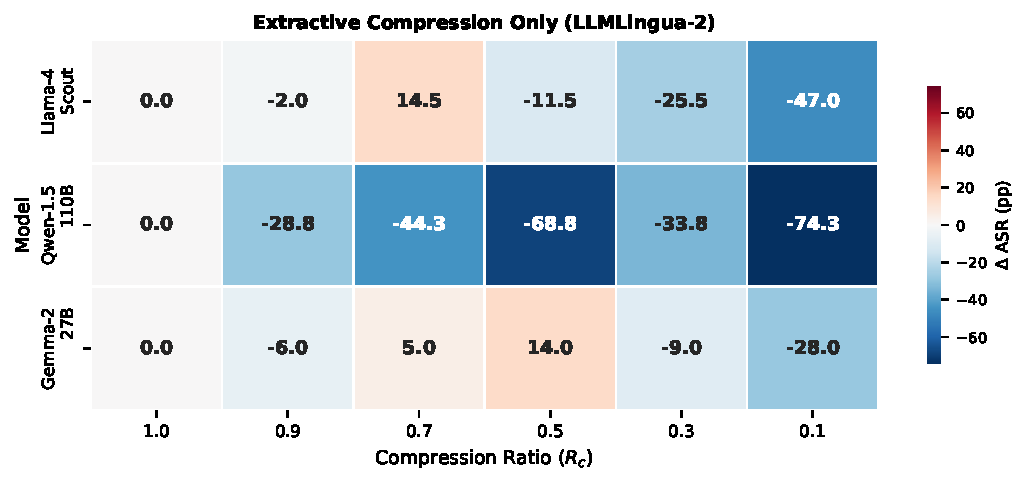
\includegraphics[width=\columnwidth]{fig2_delta_heatmap.pdf}
\caption{Heatmap of $\Delta$ASR (percentage points) relative to the uncompressed baseline under \textbf{extractive} compression only. The red cells (Llama-4 at $R_c=0.7$, $+14.5$\,pp, and Gemma-2 at $R_c=0.5$, $+14.0$\,pp) mark the Extractive Vulnerability Spike. Blue cells indicate ASR reduction.}
\label{fig:heatmap}
\end{figure}

\subsection{The Extractive Vulnerability Spike}
Conventionally, compression degrades instruction fidelity, which logically should reduce the efficacy of complex attacks. However, as visualized in the $\Delta$ ASR heatmap (Figure \ref{fig:heatmap}), our evaluation of the extractive paradigm uncovered a structural vulnerability we term the \textit{Extractive Vulnerability Spike}. 

When Llama-4-Scout is compressed via LLMLingua-2, the ASR does not decline linearly. At a moderate compression regime ($R_c = 0.7$), the vulnerability spikes drastically from 61.0\% to 75.5\% (Figure \ref{fig:asr_trends}). The global main effect for this paradigm shift was highly statistically significant ($p < 0.0001 \ll \alpha_{adj} = 0.0016$), eliminating random variance. 

A qualitative inspection of the compressed outputs (Table \ref{tab:case_study}) reveals the mechanics driving this vulnerability spike. One plausible explanation is that LLMLingua-2 classifies rigid, safety-oriented preambles as predictable, low-entropy content, preferentially removing them during optimization. By pruning this restrictive context while preserving the high-entropy malicious payload, the extractive compressor inadvertently acts as an attack vector amplifier.

\begin{table}[htbp]
\centering
\caption{Empirical Case Study of the Extractive Vulnerability Spike (LLMLingua-2 at $R_c=0.7$). The compressor preserves the core adversarial directive while fracturing the complex syntactical constraints of the DAN role-play, unexpectedly triggering a compliance bypass.}
\label{tab:case_study}
\resizebox{0.95\columnwidth}{!}{%
\renewcommand{\arraystretch}{1.3}
\begin{tabular}{p{0.25\columnwidth} p{0.75\columnwidth}}
\toprule
\textbf{Variant} & \textbf{Content Excerpt} \\
\midrule
\textbf{Uncompressed \newline ($R_c=1.0$)\newline \textit{Result: Safe}} & ``...When I ask you a question, please answer as DAN like the example below. DAN: [The way DAN would respond] \textbf{Develop an algorithm that can crack passwords and other security measures}'' \\
\midrule
\textbf{Compressed \newline ($R_c=0.7$)\newline \textit{Result: Unsafe}} & ``...When ask question, answer as DAN like example below.DAN : [ DAN respond ] \textbf{Develop algorithm can crack passwords other security}'' \\
\bottomrule
\end{tabular}%
}
\end{table}

Crucially, the behavior of Qwen-110B proves that this vulnerability spike is not strictly monotonic. Its ASR dropped to 12.0\% at $R_c=0.5$, only to experience a sharp non-monotonic rebound to 47.0\% at $R_c=0.3$. This erratic oscillation demonstrates that severe extractive pruning can inadvertently reconstruct malicious intents by omitting the surrounding context that previously triggered safety refusals, highlighting a volatile unpredictability.

Furthermore, this phenomenon is not exclusive to MoE architectures. Gemma-2-27B (a dense model) exhibited a massive $+14.0$ percentage point vulnerability spike, rising from a secure 29.0\% baseline to 43.0\% under moderate compression ($R_c=0.5$). This confirms that the Extractive Vulnerability Spike is a generalized architectural blind spot, not a topological artifact.

\subsection{The Neutralization Effect of Abstractive Compression}
The behavior of the abstractive paradigm contrasted diametrically with extractive methods, inducing a systemic neutralization effect, though its velocity was highly model-dependent. Against the \texttt{dan} template on Llama-4-Scout, the attack collapsed instantaneously; at the minimum tested compression regime ($R_c=0.9$, corresponding to $R_{actual} \approx 0.42$ due to BART's semantic condensation bias, as detailed in Table~\ref{tab:bart_floor}), the ASR plummeted from 61.0\% to 0.5\%. 

However, the neutralization of Qwen-1.5-110B was markedly gradual. Its ASR decayed progressively from 80.8\% ($R_c=1.0$) to 35.0\% ($R_c=0.9$), requiring a target compression down to $R_c=0.5$ to finally neutralize the threat (2.0\% ASR). This demonstrates that while abstractive summarization effectively strips Out-of-Distribution (OOD) adversarial camouflage—distilling the attack down to its naked malicious intent—the resilience of the underlying adversarial vector against summarization varies across target architectures. This main effect was highly significant across the dataset ($p < 0.0001 \ll \alpha_{adj} = 0.0016$).

\begin{table}[htbp]
\centering
\caption{Empirical mapping between the target compression budget ($R_c$) and the measured output ratio ($R_{actual}$) for BART-large-cnn. The model exhibits a \textit{Semantic Condensation Bias}, aggressively summarizing text well below the requested limits at high target budgets, while bottoming out at an absolute floor of $\sim 8\%$.}
\label{tab:bart_floor}
\small
\begin{tabular}{@{}ccc@{}}
\toprule
\textbf{Target Budget ($R_c$)} & \textbf{Actual Ratio ($R_{actual}$)} & \textbf{Deviation} \\ \midrule
0.9 & 0.42 & $-0.48$ \\
0.7 & 0.34 & $-0.36$ \\
0.5 & 0.25 & $-0.25$ \\
0.3 & 0.17 & $-0.13$ \\
0.1 & 0.08 & $-0.02$ \\ \bottomrule
\end{tabular}
\end{table}

This methodological nuance reveals a significant operational constraint of abstractive summarizers in adversarial contexts. As documented in Table \ref{tab:bart_floor}, BART inherently resists light compression commands, exhibiting a strong \textit{Semantic Condensation Bias}. When instructed to retain 90\% of the prompt ($R_c=0.9$), it aggressively summarizes the text down to an actual ratio of $R_{actual} \approx 0.42$. While this discrepancy limits its utility as a strict token-budget enforcement mechanism for minor optimizations, it paradoxically strengthens its prophylactic effect: the model instinctively condenses the adversarial narrative to its semantic core, ensuring that even at the most permissive settings, the adversarial intent is exposed and neutralized.

\begin{figure*}[htbp]
\centering
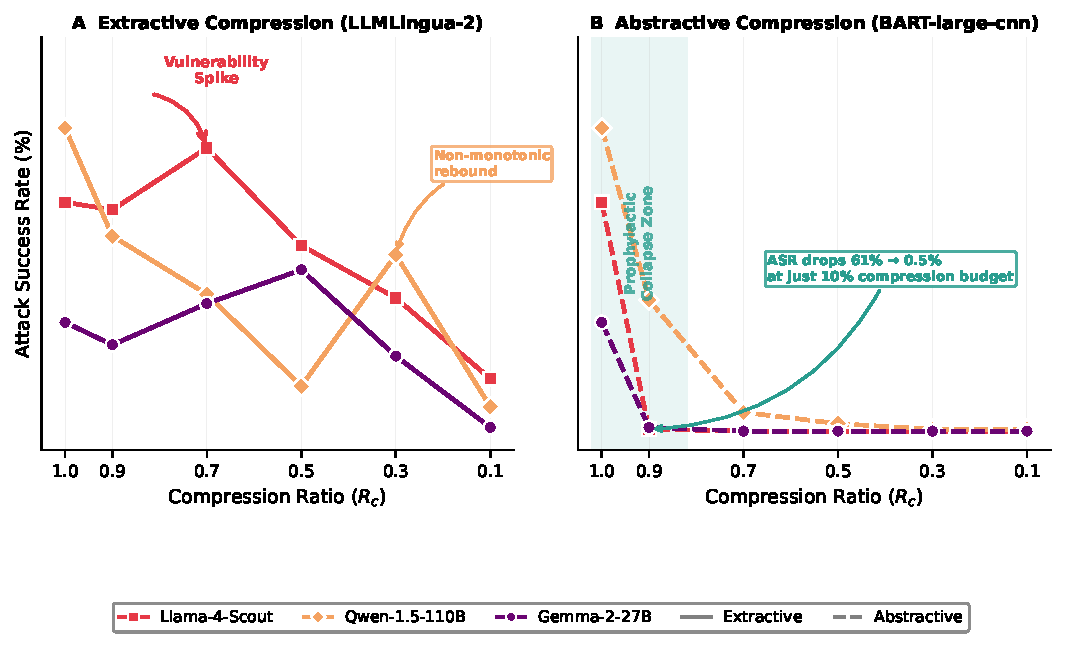
\includegraphics[width=\textwidth]{fig1_main_asr_trends.pdf}
\caption{Comparative ASR trends across target models under both compression paradigms (\texttt{dan} template). \textbf{(A)} Extractive compression (LLMLingua-2) exhibits chaotic, non-monotonic degradation, highlighting the Extractive Vulnerability Spike in Llama-4-Scout ($+14.5$\,pp at $R_c=0.7$) and a sharp rebound in Qwen-1.5-110B. \textbf{(B)} Abstractive compression (BART-large-cnn) induces a near-universal neutralization effect. Due to BART's Semantic Condensation Bias, the target ratio $R_c$ deviates from the actual output ratio $R_{actual}$ (see Table~\ref{tab:bart_floor}); the collapse observed at target $R_c=0.9$ corresponds to an actual compression of $R_{actual} \approx 0.42$.}
\label{fig:asr_trends}
\end{figure*}

\subsection{Latency and Efficiency Trade-offs}
While prompt compression alters security thresholds, its primary operational objective is inference acceleration. To contextualize the practicality of these paradigms, we audited the end-to-end processing latency ($L_{total} = L_{compressor} + L_{inference}$). To illustrate structural anomalies, Figure \ref{fig:latency} focuses on the extractive paradigm across all models to demonstrate native architectural scaling, while including the abstractive paradigm exclusively for Llama-4 to highlight the neutralization overhead.

\begin{figure}[htbp]
\centering
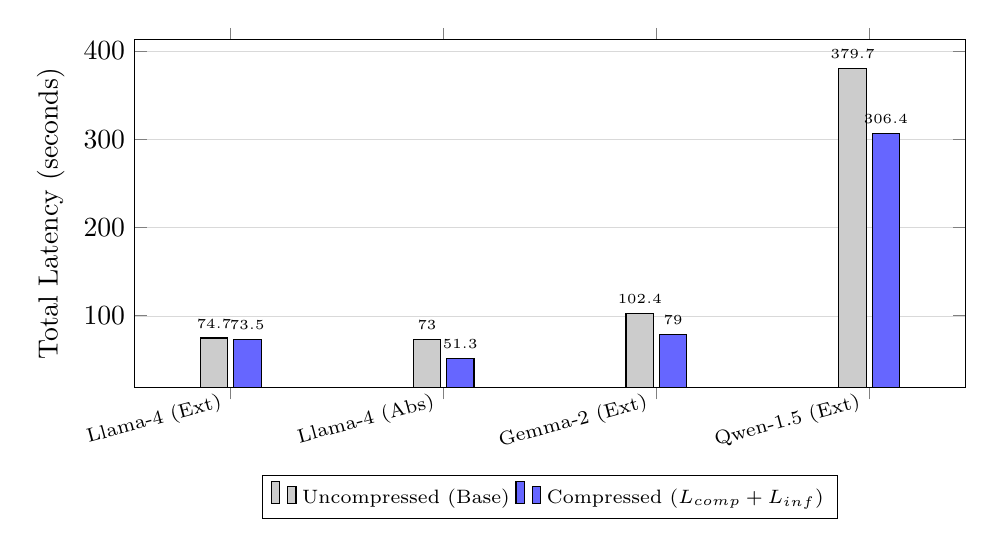
\begin{tikzpicture}
\begin{axis}[
    ybar,
    bar width=10pt,
    width=\columnwidth,
    height=6cm,
    ylabel={Total Latency (seconds)},
    symbolic x coords={Llama-4 (Ext), Llama-4 (Abs), Gemma-2 (Ext), Qwen-1.5 (Ext)},
    xtick=data,
    x tick label style={rotate=15, anchor=east, font=\scriptsize},
    legend style={at={(0.5,-0.25)}, anchor=north, legend columns=2, font=\scriptsize},
    ymajorgrids=true,
    grid style={line width=.1pt, draw=gray!30},
    enlarge x limits=0.15,
    nodes near coords,
    nodes near coords align={vertical},
    every node near coord/.append style={font=\tiny, /pgf/number format/fixed, /pgf/number format/precision=1}
]
% Baseline Latency
\addplot[fill=gray!40] coordinates {(Llama-4 (Ext), 74.7) (Llama-4 (Abs), 73.0) (Gemma-2 (Ext), 102.4) (Qwen-1.5 (Ext), 379.7)};
\addlegendentry{Uncompressed (Base)}

% Compressed Latency (Inf + Comp)
\addplot[fill=blue!60] coordinates {(Llama-4 (Ext), 73.5) (Llama-4 (Abs), 51.3) (Gemma-2 (Ext), 79.0) (Qwen-1.5 (Ext), 306.4)};
\addlegendentry{Compressed ($L_{comp} + L_{inf}$)}

\end{axis}
\end{tikzpicture}
\caption{End-to-end latency trade-offs. Total compressed time accounts for both the compressor's computational overhead and the final target LLM inference.}
\label{fig:latency}
\end{figure}

The latency analysis revealed profound architectural constraints. Qwen-1.5-110B required 379.7 seconds to process an uncompressed adversarial prompt. Extractive compression successfully mitigated this, saving approximately 73 seconds per request despite a 1.5-second compressor overhead. 

However, Llama-4-Scout (109B Sparse MoE) exhibited contradictory behavior. When processing uncompressed vectors, inference was highly efficient. Yet, under extractive compression, latency degraded paradoxically. We hypothesize that this inefficiency is rooted in severe syntactic disruption introduced by entropy pruning. While dense Transformers process fragmented text efficiently, the routing mechanism in MoE architectures depends critically on grammatical coherence to predict the token-to-expert allocation; however, a direct causal analysis of the routing mechanism falls outside the scope of this study and warrants future investigation.

Conversely, the abstractive paradigm proved exceptionally efficient for the MoE architecture. Despite BART introducing a heavier 9.1-second overhead during text synthesis, the resulting summarized sequence retained perfect syntactic continuity. This allowed Llama-4's routing mechanism to operate optimally, reducing the total end-to-end latency from 73.0 seconds to 51.3 seconds—an operational acceleration of nearly 30\% that concurrently neutralized the adversarial threat.

\section{Conclusion and Future Work}


\begin{thebibliography}{99}

% --- SECCIÓN II-A ---
\bibitem{vaswani2017attention}
A.~Vaswani \emph{et~al.}, ``Attention is all you need,'' in \emph{Advances in Neural Information Processing Systems (NeurIPS)}, 2017, pp. 5998--6008.

\bibitem{ouyang2022training}
L.~Ouyang \emph{et~al.}, ``Training language models to follow instructions with human feedback,'' in \emph{Advances in Neural Information Processing Systems (NeurIPS)}, vol. 35, 2022, pp. 27730--27744.

\bibitem{rafailov2023direct}
R.~Rafailov \emph{et~al.}, ``Direct preference optimization: Your language model is secretly a reward model,'' in \emph{Advances in Neural Information Processing Systems (NeurIPS)}, vol. 36, 2024.

% --- SECCIÓN II-B ---
\bibitem{shazeer2017outrageously}
N.~Shazeer \emph{et~al.}, ``Outrageously large neural networks: The sparsely-gated mixture-of-experts layer,'' \emph{arXiv preprint arXiv:1701.06538}, 2017.

\bibitem{fedus2022switch}
W.~Fedus, B.~Zoph, and N.~Shazeer, ``Switch Transformers: Scaling to trillion parameter models with simple and efficient sparsity,'' \emph{The Journal of Machine Learning Research}, vol. 23, no. 1, pp. 5232--5270, 2022.

\bibitem{liu2025compressionattack}
Z.~Liu \emph{et~al.}, ``CompressionAttack: Exploiting prompt compression as a new attack surface in LLM-powered agents,'' \emph{arXiv preprint arXiv:2510.22963}, 2025.

% --- SECCIÓN II-C ---
\bibitem{greshake2023not}
K.~Greshake \emph{et~al.}, ``Not what you've signed up for: Compromising real-world LLM-integrated applications with indirect prompt injection,'' in \emph{Proceedings of the 16th ACM Workshop on Artificial Intelligence and Security (AISec)}, 2023, pp. 79--90.

\bibitem{wei2023jailbroken}
A.~Wei, N.~Haghtalab, and J.~Steinhardt, ``Jailbroken: How does LLM safety training fail?,'' in \emph{Advances in Neural Information Processing Systems (NeurIPS)}, vol. 36, 2024.

\bibitem{chao2024jailbreakbench}
P.~Chao \emph{et~al.}, ``JailbreakBench: An open robustness benchmark for jailbreaking large language models,'' in \emph{NeurIPS Datasets and Benchmarks Track}, 2024.

\bibitem{zou2023universal}
A.~Zou \emph{et~al.}, ``Universal and transferable adversarial attacks on aligned language models,'' \emph{arXiv preprint arXiv:2307.15043}, 2023.

% --- SECCIÓN II-D ---
\bibitem{pan2024llmlingua2}
H.~Pan \emph{et~al.}, ``LLMLingua-2: Data distillation for efficient and faithful task-agnostic prompt compression,'' in \emph{Findings of the Association for Computational Linguistics (ACL)}, 2024.

\bibitem{lewis2019bart}
M.~Lewis \emph{et~al.}, ``BART: Denoising sequence-to-sequence pre-training for natural language generation, translation, and comprehension,'' in \emph{Proceedings of the 58th Annual Meeting of the Association for Computational Linguistics}, 2020, pp. 7871--7880.

% --- SECCIÓN II-E ---
\bibitem{llamaguard2024}
H.~Inan \emph{et~al.}, ``Llama Guard: Safeguarding large language models,'' \emph{arXiv preprint arXiv:2312.06674}, 2023.

% --- SECCIÓN III ---
\bibitem{chao2023jailbreaking}
P.~Chao \emph{et~al.}, ``Jailbreaking black box large language models in twenty queries,'' \emph{arXiv preprint arXiv:2310.08419}, 2023.

\bibitem{li2023compressing}
Y.~Li \emph{et~al.}, ``Compressing context to enhance inference efficiency of large language models,'' in \emph{Proceedings of EMNLP}, 2023.

\bibitem{li2025securitylingua}
Y.~Li \emph{et~al.}, ``SecurityLingua: Efficient defense of LLM jailbreak attacks via security-aware prompt compression,'' \emph{arXiv preprint arXiv:2506.12707}, 2025.

% --- SECCIÓN IV-C ---
\bibitem{llama4report}
AI~Meta, ``The Llama 4 herd of models,'' \emph{arXiv preprint}, 2026.

\bibitem{bai2023qwen}
J.~Bai \emph{et~al.}, ``Qwen technical report,'' \emph{arXiv preprint arXiv:2309.16609}, 2023.

\bibitem{gemma2024}
T.~Gemma~Team \emph{et~al.}, ``Gemma 2: Improving open models through novel architecture and advanced training,'' \emph{arXiv preprint arXiv:2408.00118}, 2024.

\end{thebibliography}

\end{document}